\documentclass[11pt]{report}

\special{papersize=8.5in,11in}

\topmargin -0.5in \oddsidemargin 0.00in \evensidemargin 0.00in
\textwidth 6.75in \textheight 9.0in \headheight 0.25in \headsep
0.25in \footskip 0.5in \hoffset 0in \marginparpush 0.0in
\marginparwidth 0.0in \marginparsep 0.2in

\setcounter{page}{1}

\newcommand{\D}{\displaystyle}\newcommand{\T}{\textstyle}
\newcommand{\e}{{\mathrm{exp}}}
\newcommand{\dd}{{\mathrm d}}
\newcommand{\comment}[1]{}
\newcommand{\mb}{\mathbf}
\reversemarginpar

\usepackage[final]{graphicx}
\usepackage{fancyhdr}
%\graphicspath{{Papers/}}
\usepackage{amsthm,amssymb,amsmath}
\usepackage{cite}
\usepackage{geometry}
\usepackage{amsmath}
\usepackage{booktabs}
\usepackage{color}
\usepackage{setspace}
\usepackage{subfigure}
\usepackage{url}
%\usepackage[top=2.5cm, bottom=2.5cm, right=3.5cm, left=3.5cm]{geometry}
\geometry{a4paper,scale=0.8}
\setcounter{secnumdepth}{3}

\title{Research Progress Report}

\author{Botao Zhu}

\begin{document}
	
	\maketitle
	\lhead{\sf Research Progress Report-4th} \chead{} \rhead{\sf Botao Zhu}
	\lfoot{CTRG, University of Saskatchewan} \cfoot{} \rfoot{Page \thepage}
	\renewcommand{\footrulewidth}{1.0pt}
	\renewcommand{\headrulewidth}{2.0pt}
	\renewcommand{\arraystretch}{1.3}
	\pagestyle{fancy}
	
	\renewcommand{\thesection}{\arabic{section}}
	
	\section{Reading and Research Activities}
	
	\subsection{Reading Summary}
	
	The existing networks structure and traffic control mechanisms are not adequate to cope with exponential increase in volume and complexity of the network traffic. \cite{8489985} proposed a reward based deep learning structure which jointly performs traffic load prediction and value based final action decision to control the network traffic in an intelligent manner to address the issues.
	
	\noindent For the supervised deep learning, some researchers proposed to train the network for packets forwarding based on labeled traffic data. However, the labeled traffic data are difficult to collect. In the non-supervised learning, the paths combinations are considered as the action space of the training process to choose the better action based on the action reward of each iteration. Such kind of path selection and action space design is reasonable only when the number of paths combination is finite. In order to solve the above issue, \cite{8489985} employs the set of next candidate forwarding destinations as the action space, and migrate the action decision process from the centralized controller to each distributed node. In addition, the reward are constructed as a vector to fit for the upcoming time sequences, which is able to more accurately measure the temporal connections between the selected action and get better computational cost performance than contemporary deep learning approaches.
	\begin{itemize}
		\item System model and action space format\\
		The topology of the considered network is a fully connected graph $G=\left(CR\cup AP,E\right)$, where $CR$ denotes the set of core routers in the network, $CR=\{cr_1,cr_2, \cdots, cr_{|CR|}\}$. AP denotes the set of access points, $AP=\left(ap_1,ap_2,\cdots,ap_{|AP|}\right)$, $N=|CR|+|AP|$, the total number of nodes, $E$ denotes the set of connection edges between all nodes. \\
		The action spaces is modeled and calculated as an algorithm complexity problem. Assuming the complexity of a single neural network is $\mathit{O}\left(1\right)$, The set of next-hop nodes choice is proposed as the new action space, in which, each node sets the possible next destinations as potential strategies in the action space. As the possible number of next-hop destinations of one node is $N$ at most, the upper bound of algorithm complexity of neural networks in each node is only $\mathit{O}\left(N\right)$. The time complexity of all nodes in the network is only $\mathit{O}\left(N\right)$, which is reasonable for even a complex and large scale network.
	\end{itemize}
	\begin{itemize}
		\item A joint reward and value matrix based deep learning approach\\
		In order to train the proposed next-hop destination based action space, they employ a joint training structure to construct the whole learning process as depicted in Fig.~\ref{1stfig}. Before the final action decision process, a reward matrix of each action is needed to measure the future performance after one action is selected. These rewards and value matrix are constructed as a value network to activated the second learning part called the action decision process. 
		\begin{figure}[h!]
			\centering
			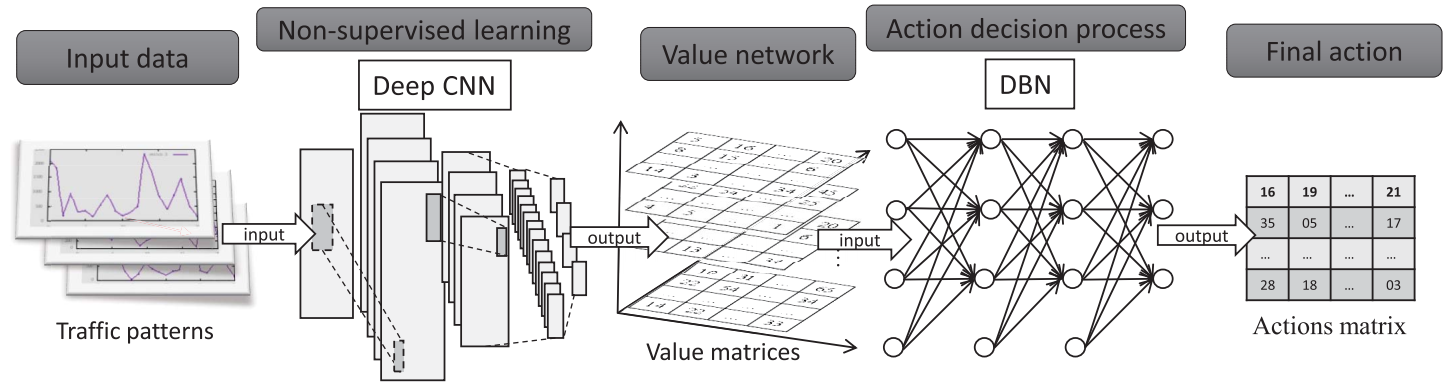
\includegraphics[width=\linewidth]{wholeprocess.png}
			\caption{The whole learning process}
			\label{1stfig}
		\end{figure}\\
	    In the learning phase, they format those features as state space and constructed with different channels as inputs, then construct the value matrix as the output. Input data can be formatted as a 3-dimensional matrix. $D_{input}=\{F,CR\cup AP,T\}$, where $F$ denotes the set of features, $T$ represents the set of time-slots. The network constructs all outputs of all nodes as a whole value matrix, shown in Fig.\ref{2ndfig}. Instead of only using a single time-slot, the output of each neural network is formatted as a future reward sequence $\{R_1,R_2,\cdots, R_n\}$, $R_i$ denotes the reward vector containing the rewards of all features in time slot $i$. $R_i = \{r^1_i,r^2_i,\cdots, r^j_i\}$, where $j$ is the number of features. 
	    \begin{figure}[h!]
	    	\centering
	    	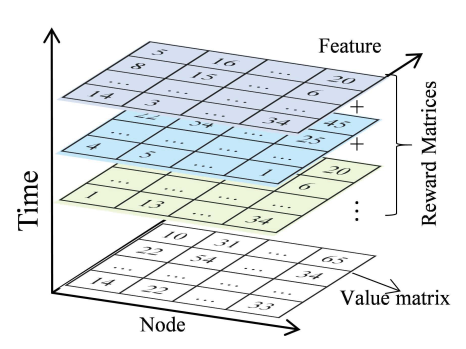
\includegraphics[width=0.7\linewidth]{matrix.png}
	    	\caption{The structure of the considered value network}
	    	\label{2ndfig}
	    \end{figure}\\
    	With the deep CNN, the connections between the spatial and temporal features between the input data are extracted by the convolutional layers. After the convolution operation, the full connection layers are used to build the connection between the extracted features and final output.\\
    	The supervised decision process is constructed with deep-DBN and the labeled training data comes from existing routing protocol. The next hop destination constructs the output data. Instead of the historical traffic pattern. They employ the value matrices as the input to activate the trained neural network. Hence, the proposed deel learning system can intelligently build the interconnections between the value network and the action space. 
	\end{itemize}
	
	
	
	\subsection{Course Summary}
	\noindent1. Finished the chapter 2, 3, 4 of Improving Deep Neural Networks and code assignments by Python, Coursera, \url{https://www.deeplearning.ai/deep-learning-specialization/ }\\
	
	\noindent2. Finished the lecture 1, lecture 2, and lecture 3 of Reinforcement Learning, University College London. \url{http://www0.cs.ucl.ac.uk/staff/d.silver/web/Teaching.html}\\

	
	\section{Objectives for the Next 2 Weeks}
	\subsection{Reading} 
	Read articles in Deep Learning for finding some novel ideas.
	\subsection{Course} 
	Study chapter 1 and chapter 2 of Convolutional Neural Networks, Coursera. \url{https://www.coursera.org/learn/neural-networks-deep-learning}
	\subsection{Code}
	Designing the following WSN model, the packets of N1 are forwarded to the next node, N3 or N4, via N2 which has a ML model. So, in this model, the routing problem can be simply simulated as a two-class problem.\\
	
	\noindent Goal:\\
	1. Learn how to build WSN by NS3 \cite{NS3}.\\
	2. Explore how to add ML model in network nodes.\\
	3. Learn how to extract network features as input layer.\\
	4. Learn how to model routing search as problems of machine learning.\\
	
	\begin{figure}[h!]
		\centering
		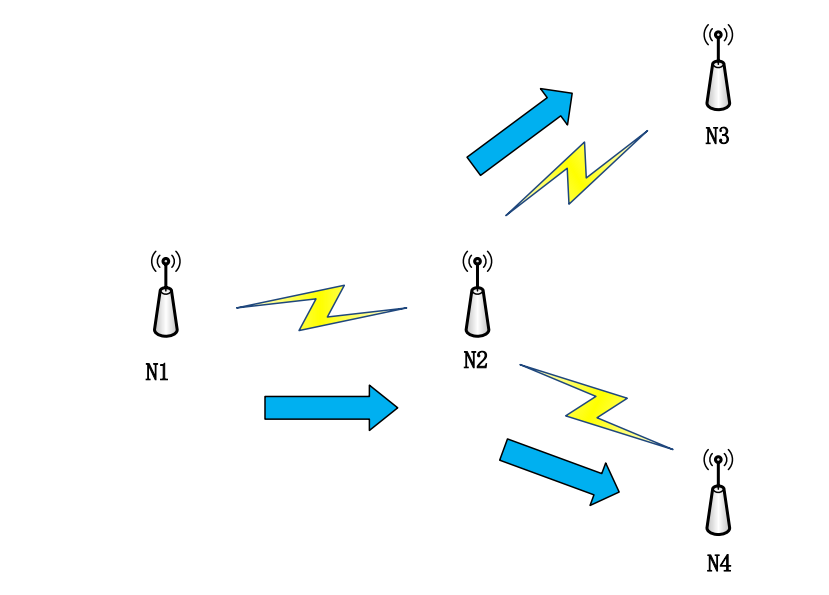
\includegraphics[width=0.8\linewidth]{wsn.png}
		\caption{ML-based WSN model}
		\label{3rdfig}
	\end{figure}

	
	\section{Advisor's Comments}
	
	\bibliographystyle{IEEEtran}
	\bibliography{janbib}
	
\end{document}